\documentclass{mcmthesis}
\mcmsetup{CTeX = FALSE,   % 使用 CTeX 套装时,设置为 true
        tcn = {\color{red}2017334}, problem = A,
        sheet = true, titleinsheet = true, keywordsinsheet = true,
        titlepage = false, abstract = true}
\usepackage{palatino}
\usepackage{lipsum}
\usepackage{epsfig} %eps文件
\usepackage{geometry}
%===============设置正文和数学字体=============================
%有些字体需要安装一些字体文件,注意辨别。
%我参照 MCM论文集的字体 使用如下宏包来定制字体。
\usepackage{caption2}

\usepackage{graphicx}
\usepackage{subfigure}
%设置段落之间的距离,若不需要删除或者注释掉即可。
\setlength\parskip{.5\baselineskip}
\newtheorem{definition}{Definition}[section]
%\def\abstractname{Summary}%可修改摘要名称

\usepackage{indentfirst}
\setlength{\parindent}{2em}

\usepackage{chngpage}
\usepackage{array}
\usepackage{booktabs}
\usepackage{threeparttable}
\usepackage{longtable}
\usepackage[numbers,sort&compress]{natbib}
%%% 实现参考文献标号在右上角
\newcommand{\upcite}[1]{\textsuperscript{\textsuperscript{\cite{#1}}}}
%然后引用的时候使用\upcite{}的格式(一般的正常引用格式为\cite{})

\usepackage{titletoc}
\titlecontents{section}[3cm]{\bf \large}{\contentslabel{2.8em}}{}{%
\titlerule*[0.5pc]{$\cdot$}\contentspage}%
\titlecontents{subsection}[4cm]{\normalsize}{\contentslabel{2.5em}}{}{%
\titlerule*[0.5pc]{$\cdot$}\contentspage}%
\titlecontents{subsubsection}[5.3cm]{\normalsize}{\contentslabel{3.0em}}{}{%
\titlerule*[0.5pc]{$\cdot$}\contentspage}%

\title{\large The Comprehensive Evacuation Planing Model in Case of Emergency}
\author{ }


\date{\today}

\geometry{left=3.0cm,right=3.0cm}

\begin{document}


\begin{abstract}



\begin{keywords}
VRP; optimal path; Tyson polygon; Time-varying curve; \\ \hspace*{1.2cm}Time-varying curve
\end{keywords}
\end{abstract}
\maketitle
%\pagestyle{empty}
\newpage                                                          %
%==================================================================
%====================生=成=目=录===================================
\begin{adjustwidth}{-1cm}{0cm}

\setcounter{tocdepth}{3}
\thispagestyle{empty}
\tableofcontents                                                  %

\end{adjustwidth}


\newpage

\pagestyle{fancy}

\setcounter{page}{1}
\section{Introduction}
\subsection{Background}
Changes in global ocean temperature will cause various marine lives to migrate. When the temperature varies too great, these animals can no longer survive and they will migrate to more suitable habitats.

herring and mackerel are very important pelagic fish in the Scottish fisheries. herring is widely distributed throughout the Northeast Atlantic, while mackerel  is mostly distributed in the North and West Seas. They are located in the deep water during the day and move towards the surface at dusk and spread over a wide area.

It has been suggested that observed spatial variation in mackerel fisheries, extending over several hundreds of kilometers, is reflective of climate-driven changes in mackerel migration patterns. 

In recent years, with the global ocean temperature rising,  the distribution of these populations has changed dramatically. However, the geographic population shift may seriously affect the disrupt the livelihood of the smaller Scottish Fisheries companies who depend on these ocean-dwelling species.



\subsection{Problem Restatement}
In order to develop the Scottish fishing industries steadily,   we need to analyze the characteristics, requirements, and interactions of herring and mackerel

1.    How does the location of herring and mackerel change according to temperature

2.    What are the best case, worse case and most likely time about  small fishing companies  based on the rate 


3.    Whether these small fishing companies should change the way they operate, what is the best way to run a small fishing company
 
4.    What will happen if a certain percentage of fishery enters the territorial seas of another country

5.    What solutions will improve the future business prospects of fishermen

\section{Assumptions}
To simplify our problems, we make the following basic assumptions, each of which is properly justified.

\begin{itemize}

\item 
Assumed that the fishing time of Scottish vessels negligible

\item 
Assumed that the ship travels in a straight line and its sailing route is from the port to the center of the position of fish.
\item 
Supposed that the salaries of crews in Scotland are equal to the average wage of the British people, at 7 pounds per hour.
\item 
Supposed the number of crew members is related to the length of the Scottish boats, about one person every two meters
\item 
Assumed that the maximum catch per vessel of a small Scottish company is 10 percent of its own weight

\end{itemize}

\section{List of Notation}

\begin{center}
\begin{longtable}{p{.1\textwidth}p{.8\textwidth}m{.4\textwidth}}
\caption{The List of Notation}\\
\hline
Symbol& Meaning \\
\hline

$L$      & The length of the Scottish vessels \\
$B$      & The width of the Scottish vessels 
                                                          \\
$D$     & The height of the Scottish vessels 
                                                        \\
$W$     & The weight of the Scottish vessels 
                                                        \\
$d$      & The   waterline length of the Scottish vessels \\
$l$       & Length between perpendiculars                                                           \\
$v$      & The average velocity  of the Scottish vessels                                            \\
$P$      & The average power of the Scottish vessels\\
$P_0$      & The average power of small Scottish vessels\\    
                                     
$V$      & The displacement of the Scottish vessels 
                                                          \\
$V_o$      & The volume of the fuel consumption
                                                          \\
$A_1$     & Total purchase cost of a Scottish vessel
                                                        \\
$A_2$       & Total salary of a crew member                                                           \\
$A_3$      & Total fuel cost of a Scottish vessel                                        \\
$A$      & total cost of a Scottish vessel                                        \\
$A_e$      &Extra cost for one voyage.  \\
$A_o$      &The total cost of a Scottish vessel   if  some proportion of fishery moves into the territorial waters of another country\\
$A_i$      &The total cost of a Scottish vessel   if  some proportion of fishery does not move into the territorial waters of another country \\
$c_1$     & The purchase cost of a Scottish vessel per hour
                                                        \\
$c_2$       & The salary of a crew member per hour                                                     \\
$c_3$      & Unit fixed cost of the ship  \\
$c_o$      &access fishing fee\\
$T_1$     & The time spent in fishing of a Scottish vessel      \\
$T_2$       & Fish preservation time at ambient temperature        \\
$T_3$     & The time spent in fishing of a Scottish vessel      \\
$T_{annual}$     & The annual avarage temperature      \\
$S$      & The distance sailed of a Scottish vessel  in the waters of another country  \\
$S_m$      & The maximum distance sailed of a large Scottish vessel that small fishing companies continue to operate out of their current  location \\
$S_o$      & The maximum distance sailed of a Scottish vessel   if  some proportion of fishery moves into the territorial waters of another country \\
$S_i$      & The maximum distance sailed of a Scottish vessel   if  some proportion of fishery does not move  into the territorial waters of another country \\
$a$      & Fish density ratio \\
$a_o$      & Oil density \\
$r_o$      & Fuel consumption ratio \\
$E$      & The earnings  of herrings and mackerels \\
$E_0$      & The small Scottish vessel's earnings  of herrings and mackerels \\
$E_1$      & The earnings  of herrings\\
$E_2$      & The earnings  of mackerels\\
$p_1$      & The price  of herrings \\
$p_2$      & The price  of mackerels  \\
$p_o$      & The price  of oil  \\
$n$      & The number  of  crews in ferries \\



 \end{longtable}
 \end{center}

 \section{The fish accumutation model}
 \subsection{basic idea}
   Below, we are going to find the trend of the yearly change and demonstrate a monthly correct and a reference expression of the spatial distribution to reach the prediction of the temperature after years, then find the relationship between temperature and the density of fishes, and finally obtain the change of fish gathering area over time. 
 \subsection{The varying temperature model}
 
  
    The changing of the sea surface temperature(SST) can be regarded as a short-term monthly average temperature change, a long-term yearly average temperature change from a time perspective; and a spatial distribution from geographical perspective. 
    We separate those changing trend by analyzing the data from project ERSST which contains 1$\deg$ resolution data from 1981 to 2010 and 2$\deg$ data from 1854 to 2020. Specificly, we use the long-term data to predicte the yearly change, and use high resolution data to be the begining of long-term prediction as well as to analyze the spatial distribution and the monthly change. The area we analyze lies in W15.5 to E13.5 and N46.5 to N65.5.
    
    

  \subsubsection{The yearly change prediction model}
    From the Long's previous work\cite{long2014fast},we know that the major factor of the yearly SST change is related to the concentration of carbon dioxide, which affact SST's retard growth model. By analyzing the yearly avarage SST of the entired area, we found an obviously increasing trend especially after 1980s. However, that model is more precise on a time scale of hundreds of years, and we found a quadratic model is more accurate to predicte the temperature on a time scale over years, fitting the rising segment of the logistic curve, especially with the concider that the concentration of carbon dioxide are only dramatic growth in recent decades and affect the retard growth model. 
   
    The quadratic predicted function is:
    \begin{equation}
        8.526*10^{-5}*(t-1840)^2-1.327*10^{-2}*(t-1840)+1.017*10^1
    \end{equation}
    
    The logistic predicted function is:
    \begin{equation}
      \frac{15.00}{1+(\frac{15.00}{8.615}-1)e^{-0.0026*(t-1822)}}
    \end{equation}

    \begin{figure}[htbp]
      \centering{
      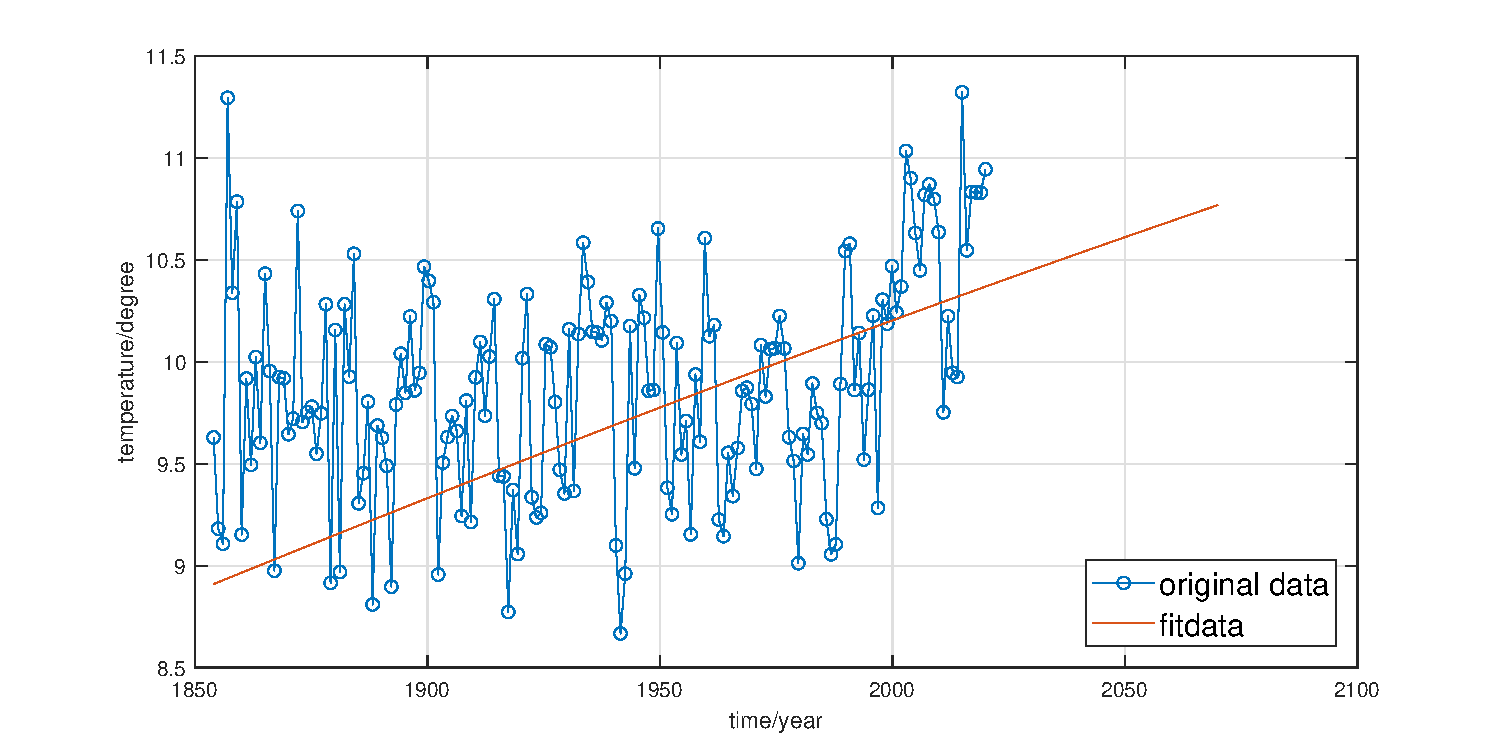
\includegraphics[width=0.9\textwidth]{image/predic_log.eps}}
      \caption{using logistic model}\label{figure1}
    \end{figure}
    \begin{figure}[htbp]
      \centering{
      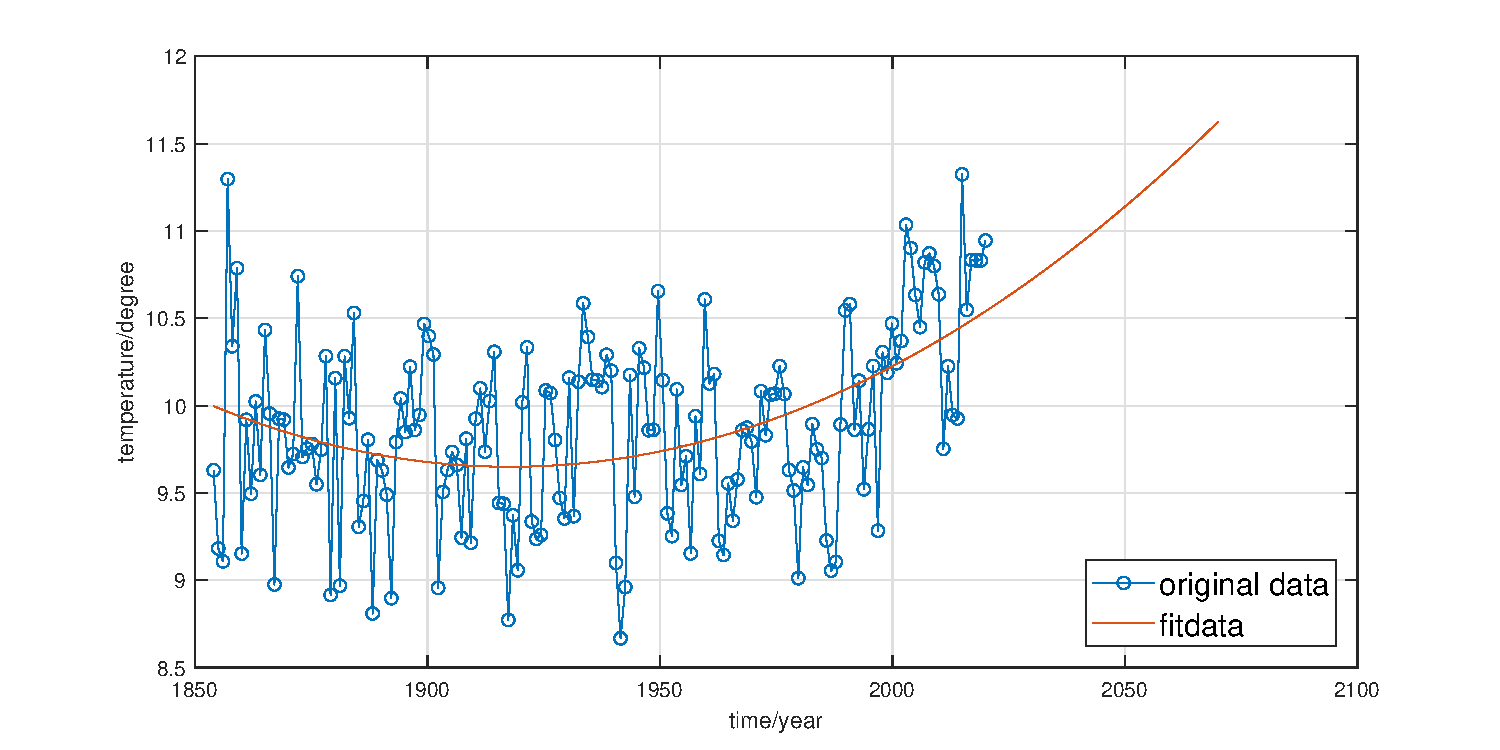
\includegraphics[width=0.9\textwidth]{image/predic_qua.eps}}
      \caption{using quadratic model}\label{figure1}
    \end{figure}
    
  
    
  \subsubsection{Monthly correct of the prediction}
    The monthly or even dayly rate of SST change is much stronger than the rate of yearly SST change and is important to the analysis of the fishes distrbution. In our model, we assume that the monthly change has a central value related to its annual avarage temperature. We also assume that the monthly change are determined by the seasonal change and independent of the factors which affect the yrarly change of avachange temperature. Then we are going to use the predicted annual avarage temperature above and add a monthly correction to get the actual temperature accurate to month. 
    A long-term dayly avarage and a spatial avarage are made based on SST data from 1981 to 2010 in the area we Analyzed. Since the seasonal change of temperature are mostly related to the rotation of the earth, it is convenience to suppose this change has a trigonometric form. And we find the monthly correction is: 
    \begin{equation}\label{}
      T(t)=3.3598\sin(-0.0184t+0.5921\pi)+0.1382+T_{annual}      
    \end{equation}
    where $T_{annual}$ is the annual avarage temperature, and t is days ranging from 1 to 365.
    To simplicity the representation, our further work are still using the annual avarage temperature, which as actually close to the temperature in spring and fall, as the beginning of the yearly prediction model. The affect of the seasonal change will be considered in the profit model, which will be discussed in later section. 

    \begin{figure}[htbp]
      \centering
      \subfigure[spatial temperature distribution]{
      \begin{minipage}[t]{0.5\linewidth}
      \centering
      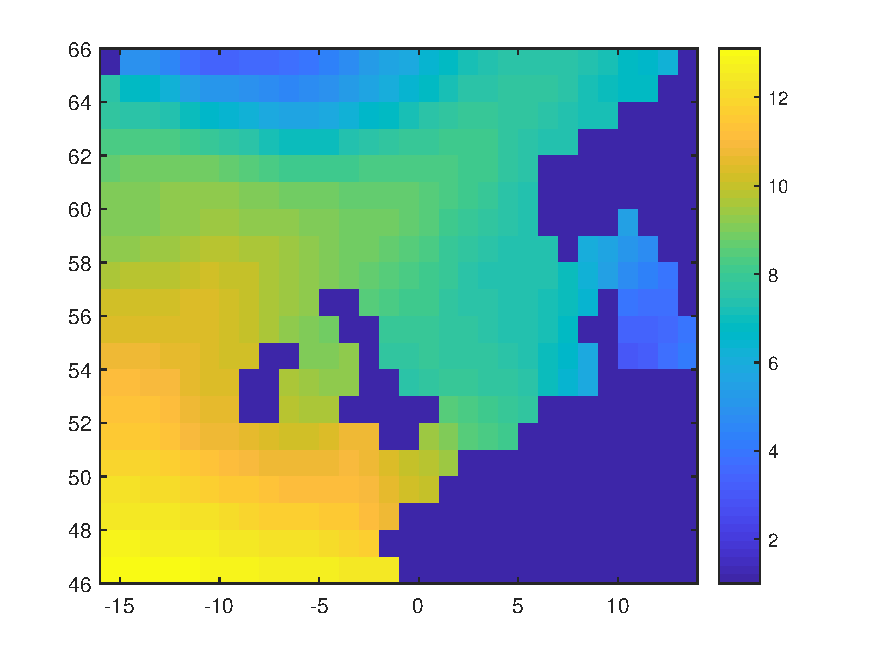
\includegraphics[width=3in]{image/general_distribution.eps}
      %\caption{fig1}
      \end{minipage}%
      }%
      \subfigure[monthly changing and fit]{
      \begin{minipage}[t]{0.5\linewidth}
      \centering
      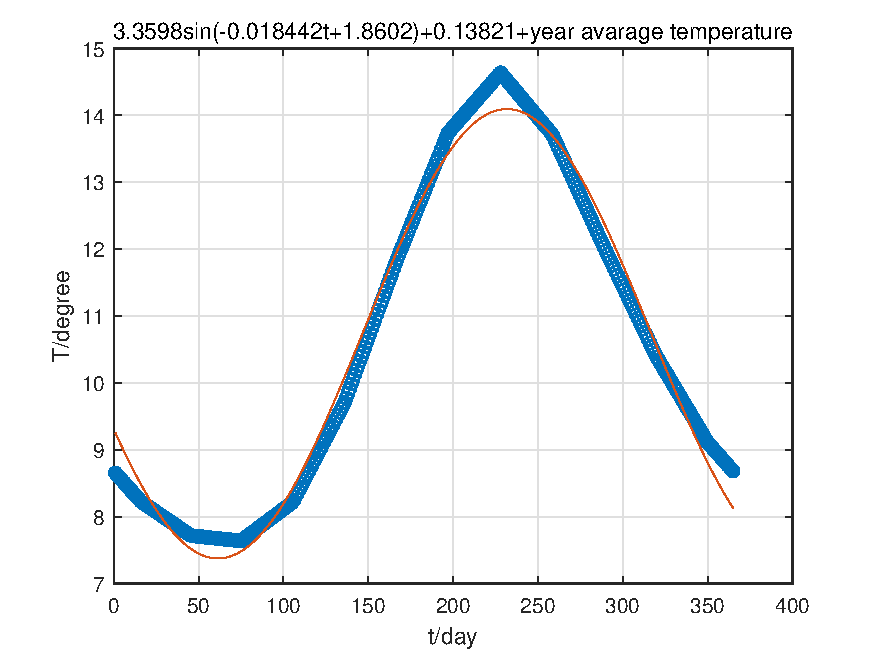
\includegraphics[width=3in]{image/month_correct.eps}
      %\caption{fig2}
      \end{minipage}%
      }
      
      \centering
      % \caption{}
    \end{figure}

  \subsubsection{Spatial distribution model}
    During the work above, we make a spatial avarage of the data,but we are also interseted in the spatial distribution of the SST. From jansen's work\cite{jansen2012migration}, the SST of a given location in Scottish area are strongly related to the distance between that place and the continental shelf. In our model, we assume that those dependencies of distance can be converted into the dependencies of longitude and latitude. We also assume this distribution is damping from the mean temperature value of the area at a given time, which offers a way to predict the future's SST distrbution based on the predicted value of annual avarage SST. 
    The equation we obtain is:

    \begin{equation}\label{}
      T(t)=-0.34\sqrt{(Lon+14.08)^2+(Lat+104.87)^2}+T_{annual}+55.65      
    \end{equation}
    where $T_{annual}$is the annual avarage temperature.
    \begin{figure}[htbp]
      \centering
      \subfigure[fit of the spatial temperature distribution]{
      \begin{minipage}[t]{0.5\linewidth}
      \centering
      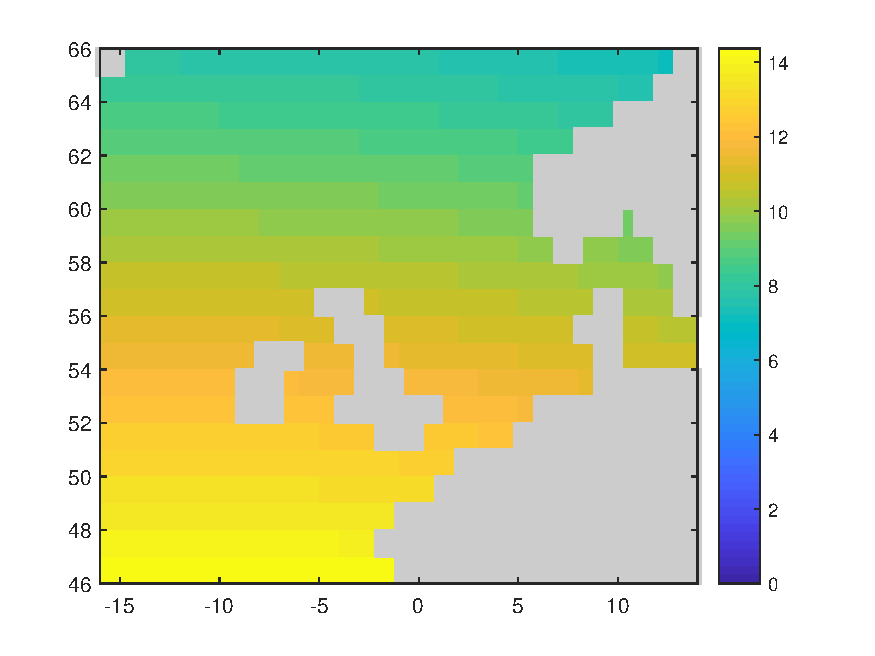
\includegraphics[width=3in]{image/spatial_distribu_fit.eps}
      %\caption{fig1}
      \end{minipage}%
      }%
      \subfigure[relative error of fit]{
      \begin{minipage}[t]{0.5\linewidth}
      \centering
      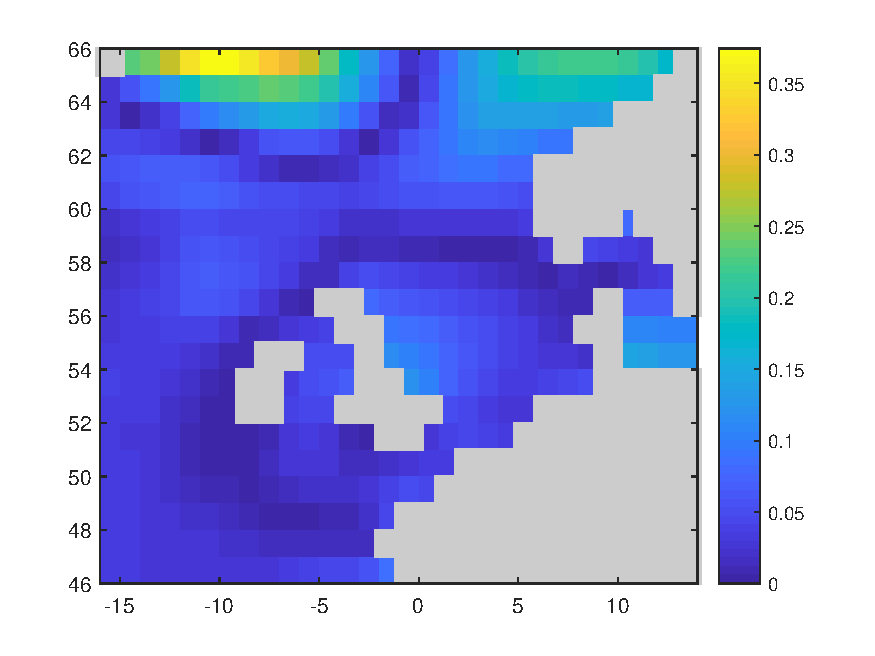
\includegraphics[width=3in]{image/spatial_distribu_fit_err.eps}
      %\caption{fig2}
      \end{minipage}%
      }
      
      \centering
      % \caption{}
    \end{figure}
    
    However, in order to reduce the error, we will not use that analytical method, but based on the original spatial distribution data which we used to get this analytical representation. 

 \subsection{The fish-temperature model}
  As we known, fish need the proper habitat to service, and temperature play an important role in multiply of fish, such as the mackerel population is found further upstream in warmer waters as the current cools through winter\cite{jansen2012migration}. In our previous predictions, the increase of  SST because global warming is obvious, so we take fisheries data  from The International Council for the Exploration of the Sea(ICES) and make a comparison. 

 \begin{figure}[htbp]
 \centering{
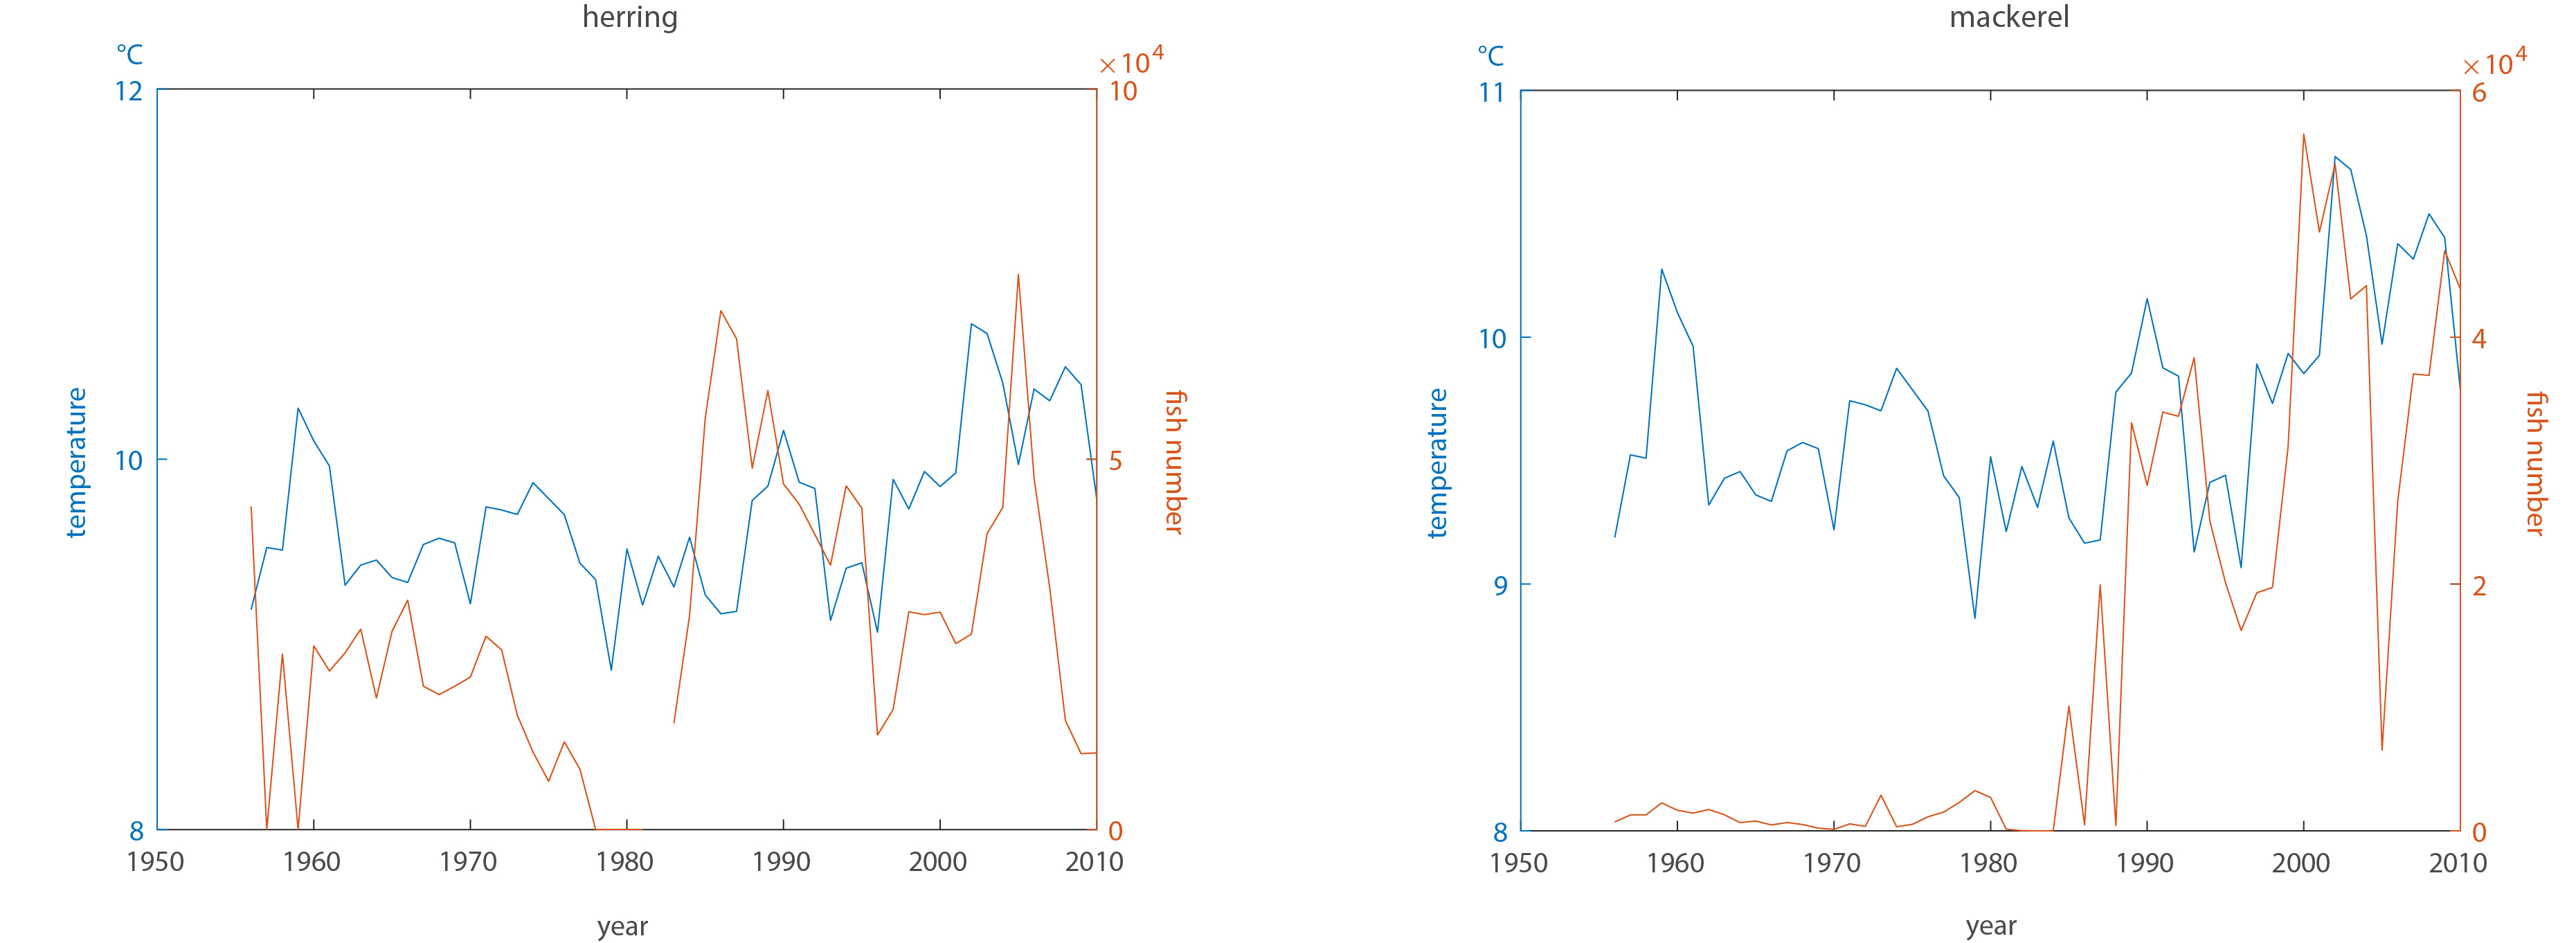
\includegraphics[width = .8\textwidth]{picture/fish-temp.jpg}}
\caption{Comparison graph}\label{figure1}
 \end{figure}

  According to the graph, we can tell that besides fisheries productivity growth and some statistical gaps, the density of fish is particularly relevant to SST. So we use Pearson correlation coefficient to correlation analysis. 

  \begin{table}[h]
    \centering
    \setlength{\abovecaptionskip}{0pt}%
    \setlength{\belowcaptionskip}{15pt}%
    \caption{The result of correlation analysis}
    \begin{tabular}{ccccccccc}
    \toprule[1.5pt]
    result &herring &mackerel\\
    \toprule[1.5pt]
    r&0.4637&0.5463\\
    \bottomrule[1.5pt]
    \end{tabular}
  \end{table}

  So it's highly correlative. Then we use them to fitting the Gaussian distribution, and get the desired relationship between temperature and fish density.

 \begin{figure}[htbp]
   \centering{
   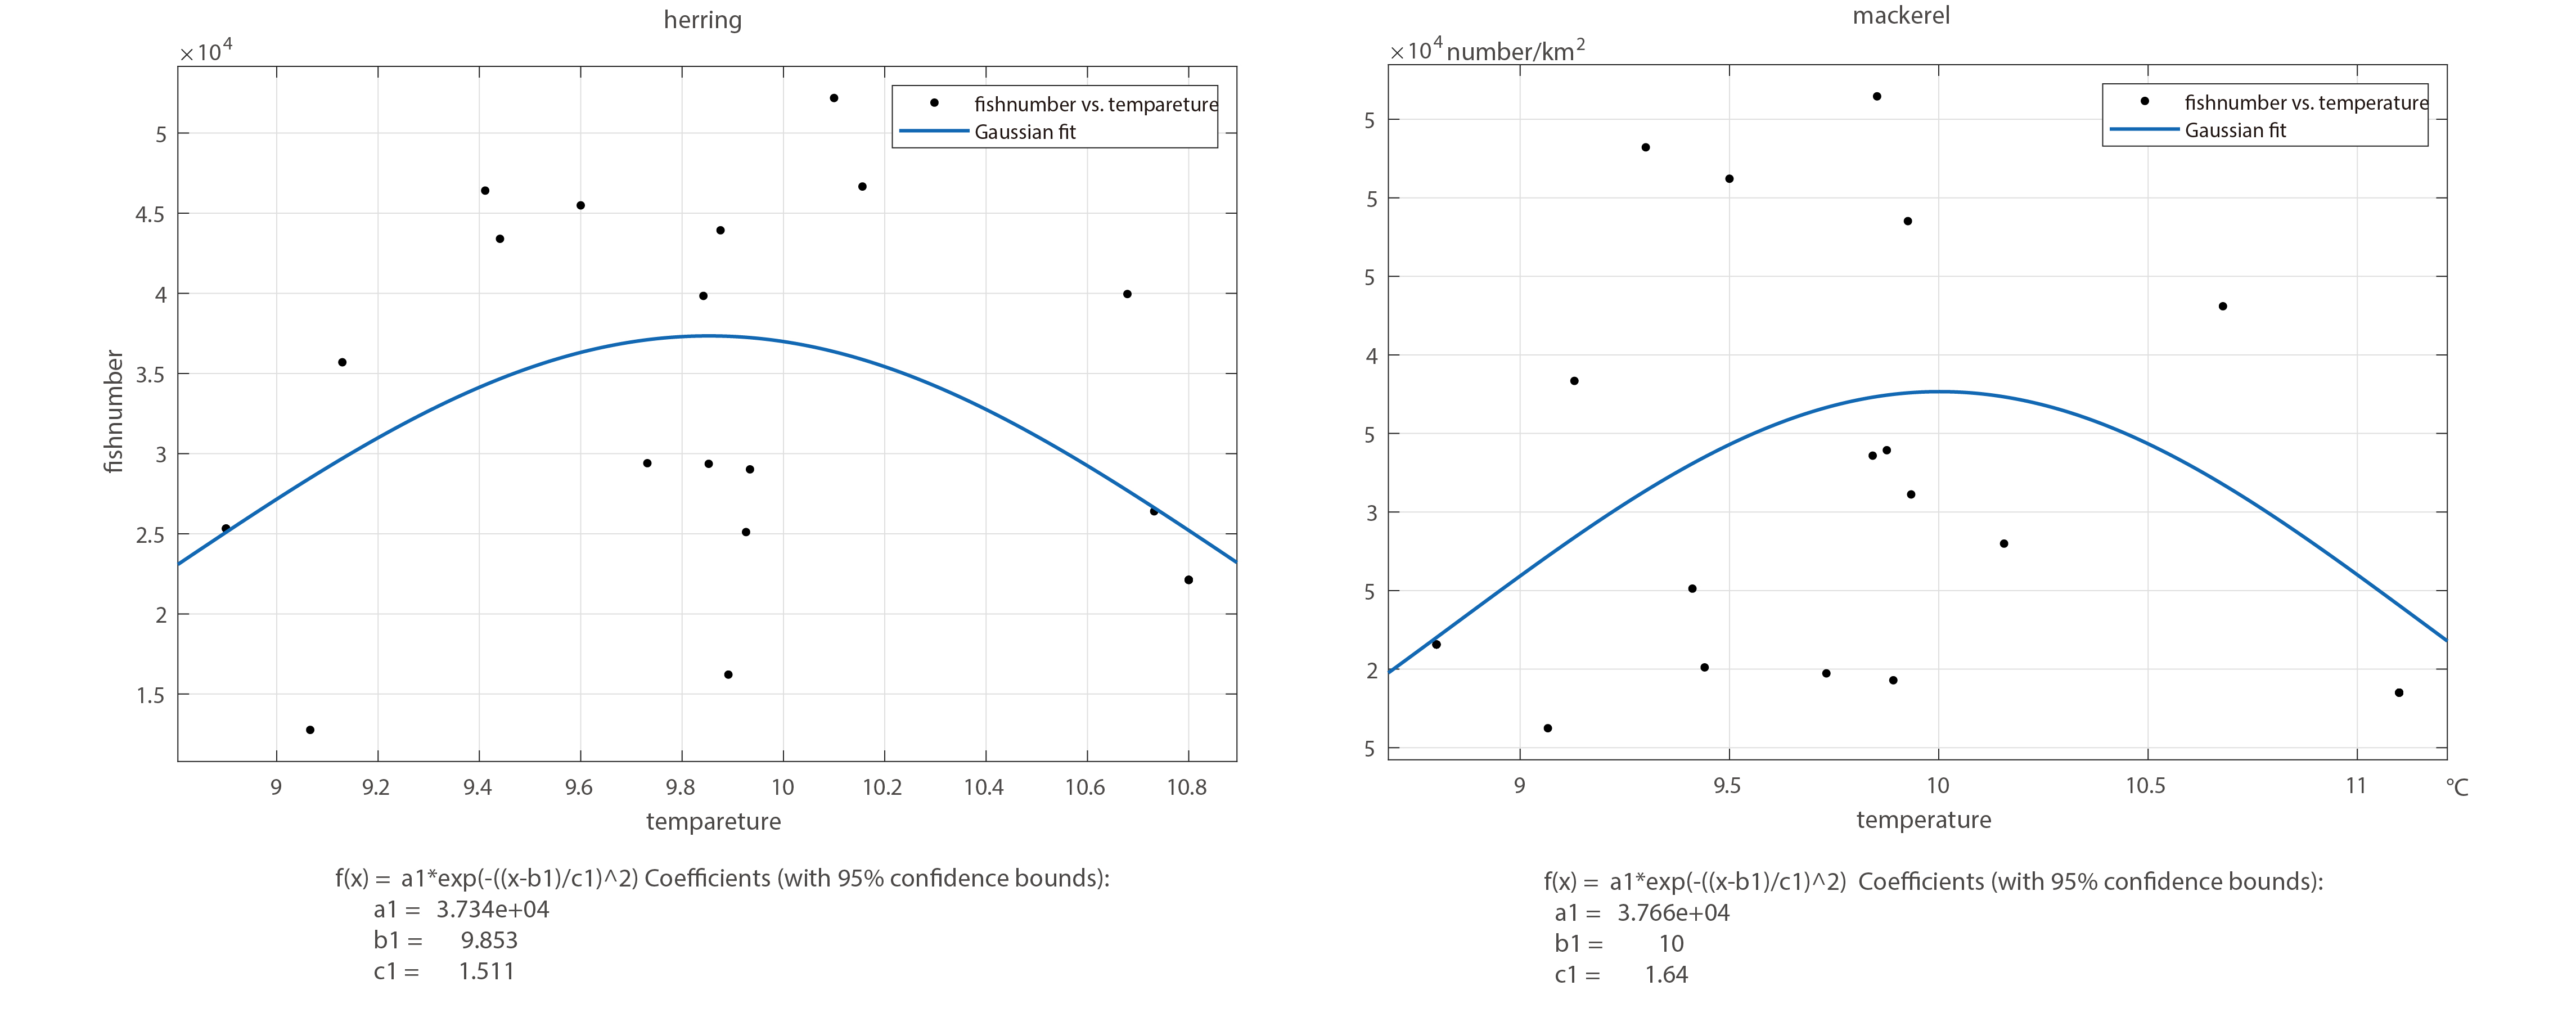
\includegraphics[width = .8\textwidth]{picture/fish-temp_fitting.jpg}}
   \caption{Fitting result}\label{figure1}
 \end{figure}

\subsection{The prediction of fish accumutation distribution}
  We have obtained the relationship between fish density and temperature as well as the basic model to caculate the temperature distribution in the future. The following figure are going to reveal the sea surface temperature distribution and fish accumulation area in the current and after 10,25,50 years. 

\begin{figure}[htbp]
  \centering

  \subfigure[fish accumulation areas after 0 years]{
  \begin{minipage}[t]{0.5\linewidth}
  \centering
  \includegraphics[width=2.5in]{image/fish_area_after0years.eps}
  %\caption{fig1}
  \end{minipage}%
  }%
  \subfigure[fish accumulation areas after 10 years]{
  \begin{minipage}[t]{0.5\linewidth}
  \centering
  \includegraphics[width=2.5in]{image/fish_area_after10years.eps}
  %\caption{fig2}
  \end{minipage}%
  }%
  \quad
  \subfigure[fish accumulation areas after 25 years]{
  \begin{minipage}[t]{0.5\linewidth}
  \centering
  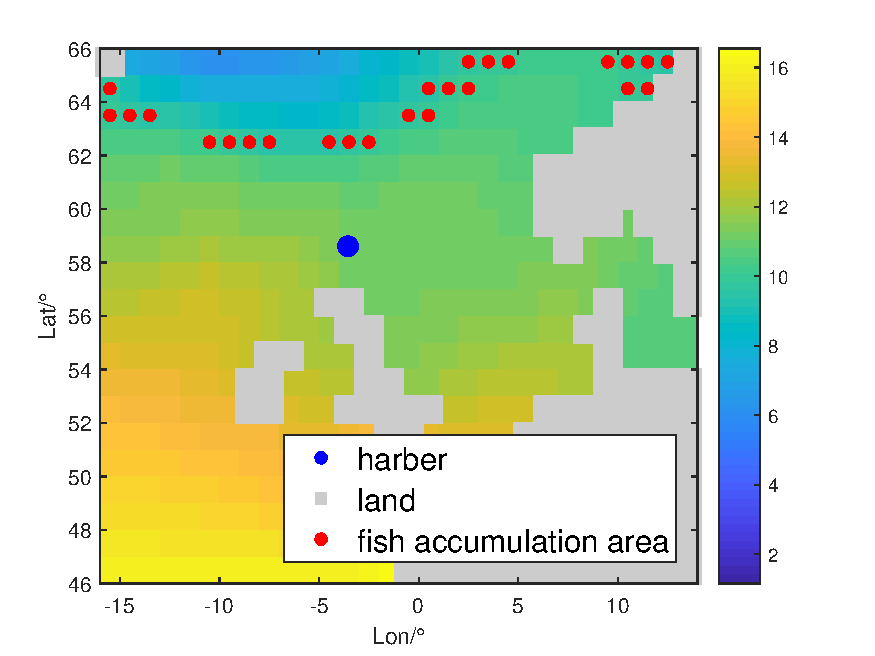
\includegraphics[width=2.5in]{image/fish_area_after25years.eps}
  %\caption{fig1}
  \end{minipage}%
  }%
  \subfigure[fish accumulation areas after 50 years]{
  \begin{minipage}[t]{0.5\linewidth}
  \centering
  \includegraphics[width=2.5in]{image/fish_area_after50years.eps}
  %\caption{fig2}
  \end{minipage}%
  }
  \centering
  \caption{fish accumulation areas}
\end{figure}

\section{The Distribution Model}
\subsection{Initial costs and profits}
\begin{figure}[ht]
  \centering{
  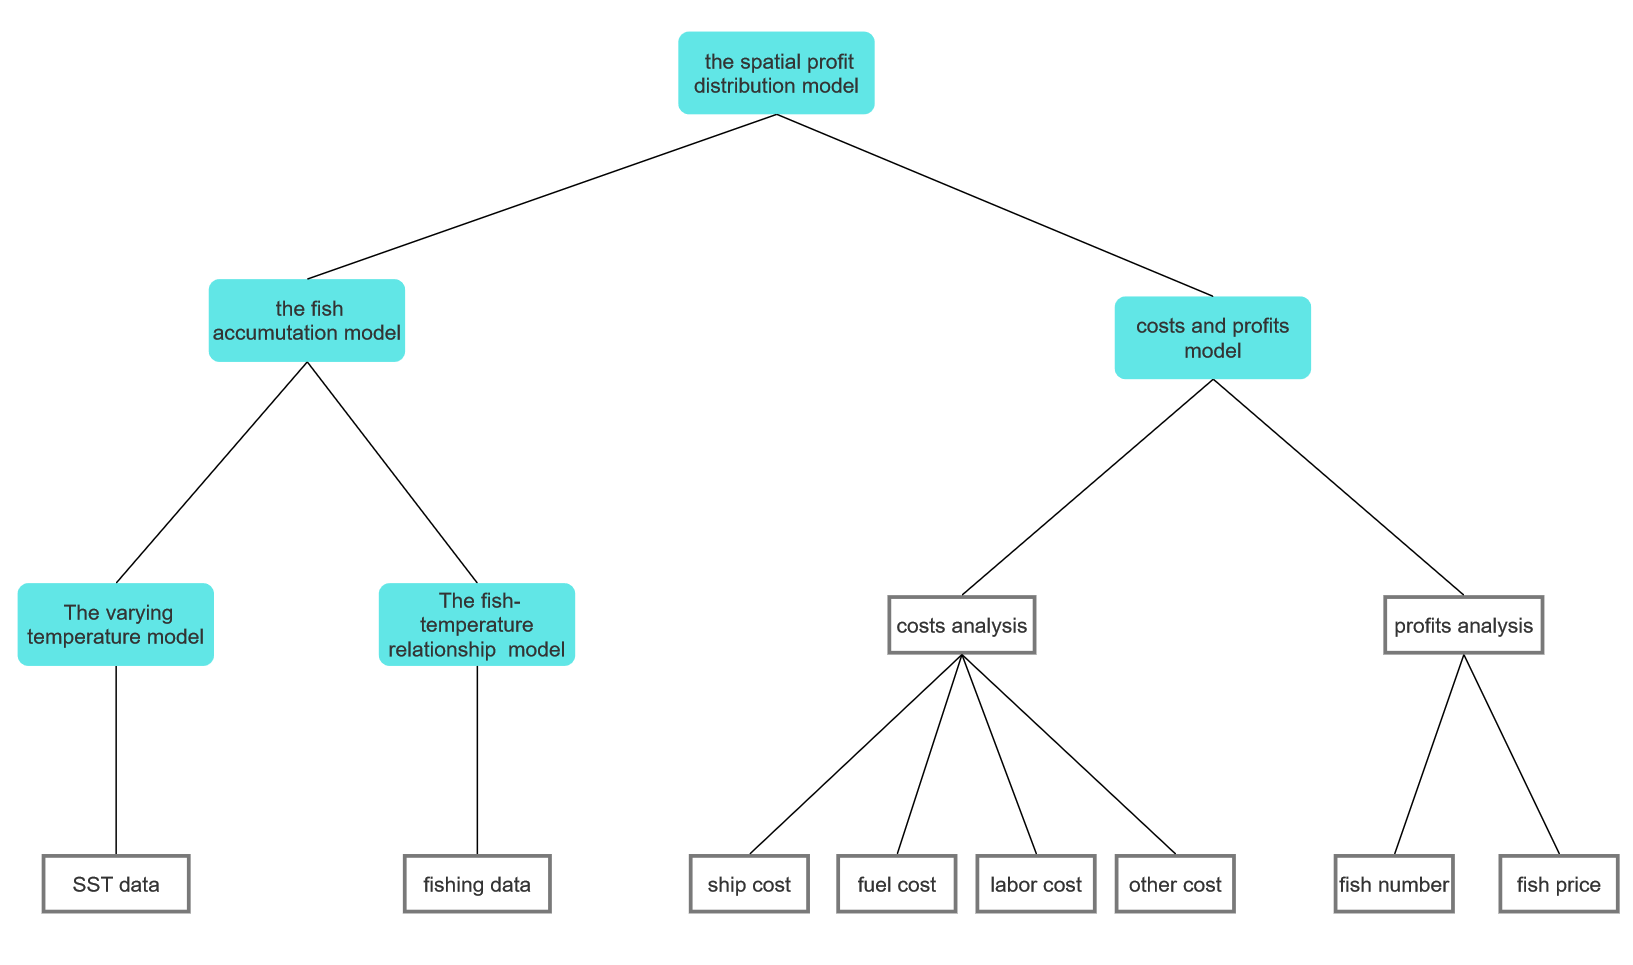
\includegraphics[width=0.8\textwidth]{./picture/figure1.png}}
  \caption{the spatial profit distribution model}
\end{figure}


As can be seen from the 2016 Scottish Marine Statistics (Table 3), most of the Scottish vessels that capture herring and mackerel are larger than 40 meters in length. Figure 6 is the structural model of the ship. We simplified the structure of the ship to a cuboid, and the relationship between its length, width, and height is shown in Table 3. We assume that the length of the Scottish vessels in small company is about 40 meters, the width is one quarter of its length, the height of the waterline is one twelfth of the length, and the length between the  perpendiculars  is equal to the length of the boat.

\begin{table}[!htb]
  \centering
  \setlength{\abovecaptionskip}{0pt}%    
  \setlength{\belowcaptionskip}{15pt}%
  \caption{The range dimension ratios of  trawlers}
  \begin{tabular}{ccccccccc}
  \toprule[1.5pt]
  parameter &L/B&B/d&D/d\\
  \toprule[1.5pt]
  Range of steel materials&3.93-5.00&2.38-3.65&1.19-1.38\\
  Range of wood materials&3.19-4.53&2.61-4.67&1.06-1.44\\
  \bottomrule[1.5pt]
  \end{tabular}
  \end{table}

From Table 4, it is estimated that the average power of a 40-meter-long Scottish vessel is 4000 kilowatt and. the average tonnage is about 1300 tonnes. Considering the fishing and netting time of Scottish vessels  $T_0$, it can.be assumed around two hours. So the speed and flight time are calculated from the speed-related formula.



\begin{table}[!htb]
\centering
\setlength{\abovecaptionskip}{0pt}%    
\setlength{\belowcaptionskip}{13pt}%
\caption{The prices of two species : 2012 to 2016}
\begin{tabular}{ccccccc}
\toprule[1.5pt]
Year&2012&2013&2014&2015&2016&average\\
\bottomrule[1.5pt]
Herring (pound  per tonne)  &565&408&308&369&665&463\\
Mackerel (pound  per tonne)  &1034&979&832&664&895&880.8\\
\bottomrule[1.5pt]
\end{tabular}
\end{table}


\begin{table}[!htb]
\centering
\setlength{\abovecaptionskip}{0pt}%    
\setlength{\belowcaptionskip}{13pt}%
\caption{The information about Scottish registered vessels}
\begin{tabular}{ccccccc}
\toprule[1.5pt]
vessel length (metres)&<=10&10-12&12-15&15-24&24-40&>=40\\
\bottomrule[1.5pt]
Herring (tonnes)&0&0&0&7&1505&63031\\
Mackerel (tonnes) &811&0&0&42&3802&183831\\
Average tonnage (tonnes)&4&13&22&110&273&1748\\
Average age (year)&26&33&29&31&28&17\\
Average engine power (kW)&57&127&190&325&641&4327\\

\bottomrule[1.5pt]
\end{tabular}
\end{table}

\begin{figure}[tbp]
  \centering{
  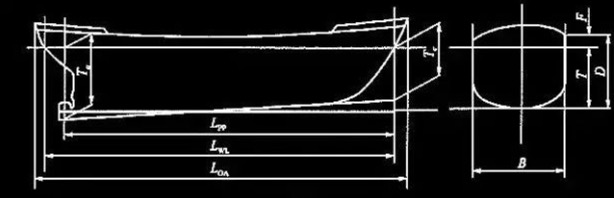
\includegraphics[width=1\textwidth]{./picture/figure2.jpeg}}
  \caption{a ship model}\label{figure1}
\end{figure}

\begin{equation}
\left\{
\begin{array}{lr}
v=1.84\times \ (\frac{P}{V}) ^{0.237} \times \sqrt{l} &\\
l \approx L= 40 &\\
P=4000&\\
V=L\times B\times\ d =\frac{1}{48\times L^3}\\
\end{array}
\right.
\end{equation}

\begin{equation}\label{5}
T=\frac{S}{v}
\end{equation}


\begin{equation}\label{5}
A_1=c_1 \times T_1
\end{equation}

\begin{equation}\label{6}
<<<<<<< HEAD
A_2=c_2  \times( T_1+T_0)  \times n =c_2  \times( T_1+T_0) \times L \times  \frac{1}{2}
=======
A_2=c_2  \times T_1 \times L \times  \frac{1}{2}
>>>>>>> 0ffe63186d781ab73ee1b7603ae82230433a53f3
\end{equation}

\begin{equation}\label{7}
A_3=V_o  \times p_o
\end{equation}

\begin{equation}
\left\{
\begin{array}{lr}
V_o=r_o \times P \times T_1 \times a_o &\\
a_o=0.8&\\
p_o=0.5&\\
A_3=V_o  \times p_o\\
\end{array}
\right.
\end{equation}





\begin{equation}\label{8}
A=A_1+A_2+A_3+A_e
\end{equation}

Where:

$A_1$ represents the average working cost per hour of the large Scottish vessel.As a Scottish vessel with a length of 40 meters, the purchase price is approximately 44,000 pounds, the number of days of operation is 180 days per year, and the daily working time is 13 hours.

$A_2$ is the cost that the small company need to pay about 20 crew members during a voyage

$A_3$ is the cost about fuel for one voyage

$A_e$ is a fixed cost of about 20,000 pounds for a small sailing company in Scotland, including depreciation fees for fishing boats, fishing nets, hook fees, port fees, and loss costs during the off-season.
 


\begin{equation}
\left\{
\begin{array}{lr}

E_1=1300 \times 10\% \times a_1 \times p_1 &\\
E_2=1300 \times 10\% \times a_2 \times p_2 &\\
E= \frac{a_1 \times p_1}{a_1 \times p_1+ a_2 \times p_2} \times E_1 + \frac{a_2 \times p_2}{a_1 \times p_1+ a_2 \times p_2} \times E_2\\

\end{array}
\right.
\end{equation}

The weighted average prices and the proportion of density in different regions of herring and mackerel  is used to calculate the earnings of small Scottish companies during a voyage. 

Since no refrigerant fishing, in order to ensure fresh fish, the sum of the return time and fishing and netting time  of Scottish vessel must be shorter than the fresh-keeping period of the fish, $T_2$, around 20 hours.

\begin{equation}\label{10}
\frac{T_1}{2}\leq T_2
\end{equation}



\subsection{the spatial profit distribution model}
  We have obtained the predicted fish density distribution in last section, and after the work above we can calculate the net profit by the sailing cost, the gross profit from fishing, and a constant cost appears on every voyage.
  
Ignoring national territorial limits, it can be seen from the figure(a) and (b) that there is no obvious change in the income of fishing in 10 years, which is because the slow increase of sea temperature has a time lag to the migration of fish. After 25 years (c), the largest income gradually migrates northward. Fifty years later, the school of fish is obviously moving north. At this time, the port is far from the school of fish, and the fishing cost will increase significantly (d)

\begin{figure}[htbp]
  \centering

  \subfigure[spatial net profit distribution after 0 years]{
  \begin{minipage}[t]{0.5\linewidth}
  \centering
  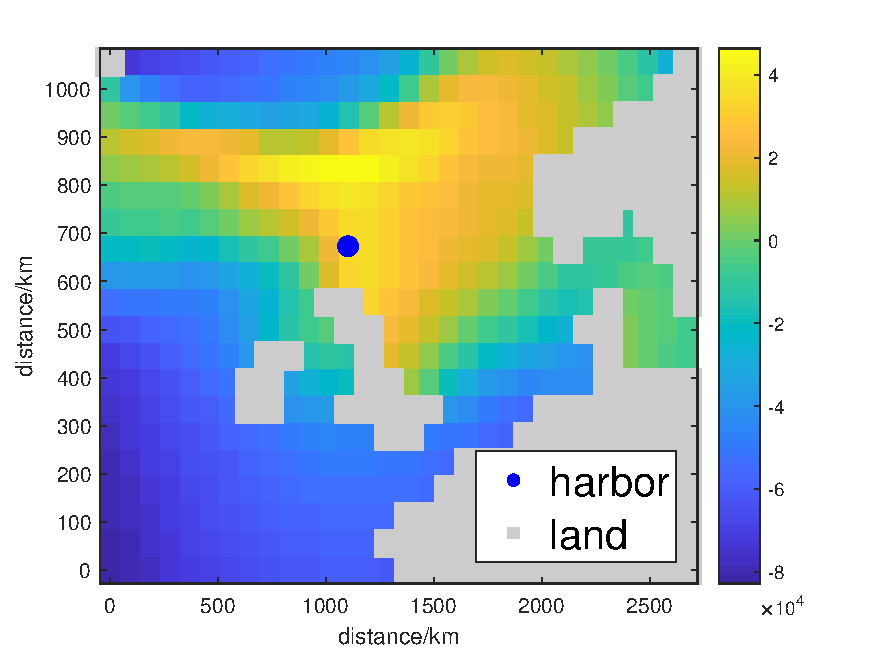
\includegraphics[width=2.5in]{image/profit_dis_afterqua0image.eps}
  %\caption{fig1}
  \end{minipage}%
  }%
  \subfigure[spatial net profit distribution after 10 years]{
  \begin{minipage}[t]{0.5\linewidth}
  \centering
  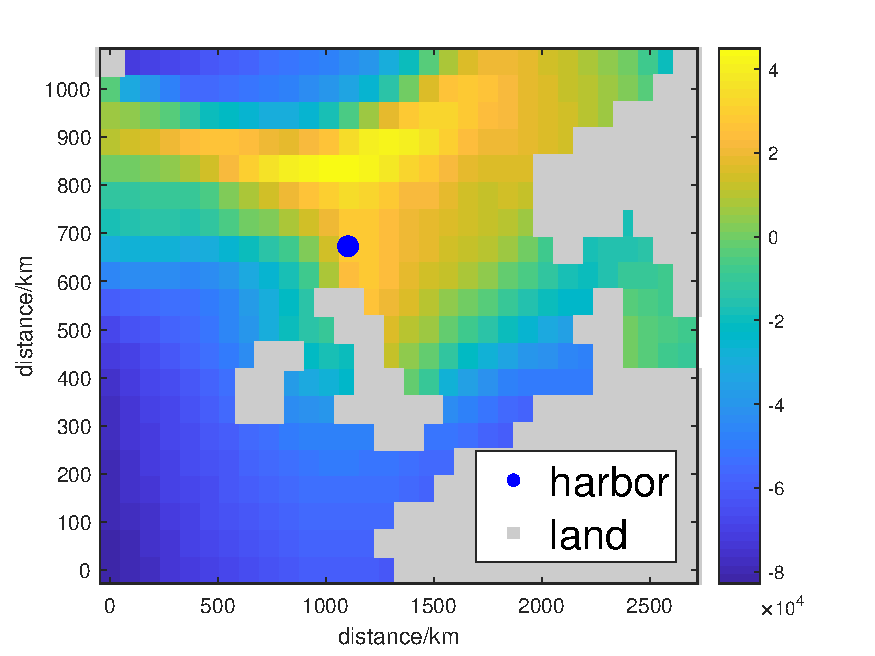
\includegraphics[width=2.5in]{image/profit_dis_afterqua10image.eps}
  %\caption{fig2}
  \end{minipage}%
  }%

  \quad
  \subfigure[spatial net profit distribution after 25 years]{
  \begin{minipage}[t]{0.5\linewidth}
  \centering
  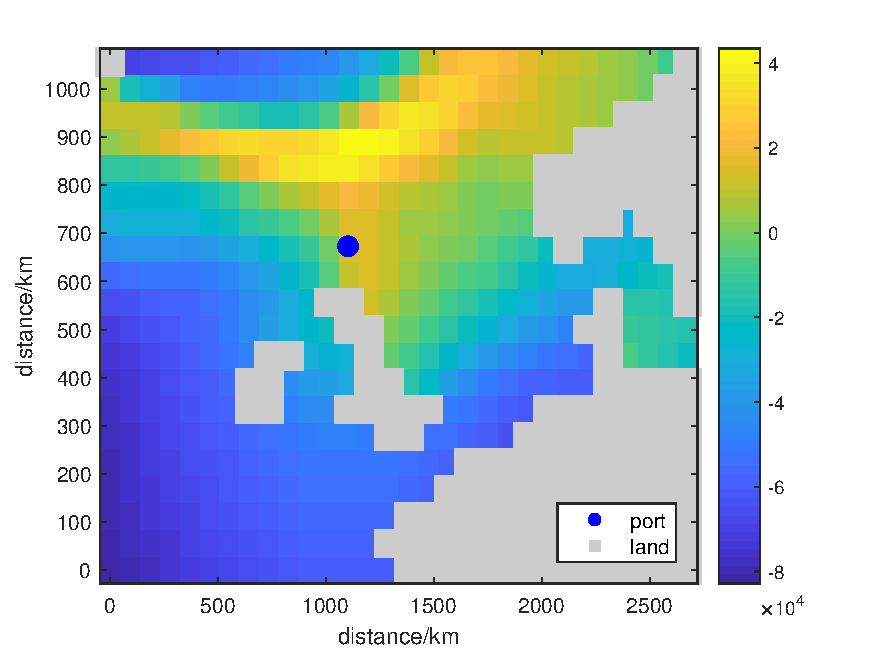
\includegraphics[width=2.5in]{image/profit_dis_afterqua25image.eps}
  %\caption{fig1}
  \end{minipage}%
  }%
  \subfigure[spatial net profit distribution after 50 years]{
  \begin{minipage}[t]{0.5\linewidth}
  \centering
  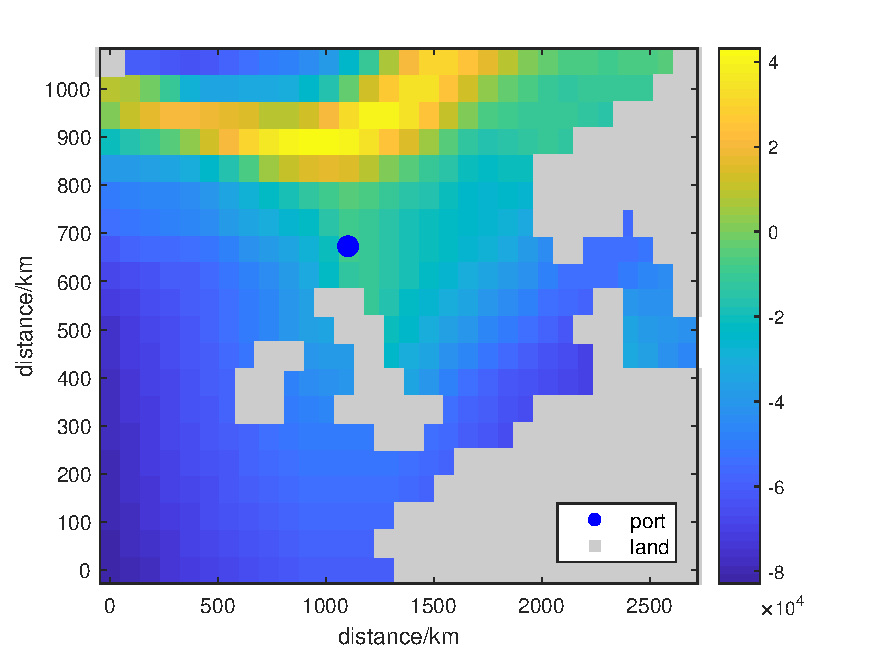
\includegraphics[width=2.5in]{image/profit_dis_afterqua50image.eps}
  %\caption{fig2}
  \end{minipage}%
  }
  \centering
  \caption{spatial net profit distribution}
\end{figure}

Due to the limitation of fish preservation time,  Scotland small company can make a large profit offshore. From the comparison about the offshore distance and income (e), it can be concluded that when the distance is less than 200 kilometers, the company's profit is positively related to the density of the local fish school. There are obvious differences in various years, because the fish school moves northward with the change in temperature. As can be seen from the figure (f) that after about 40 years, the net profit will drop to 0. Therefore, these small companies should take measures in advance to deal with changes in fish stocks.

\begin{figure}[htbp]
  \centering
  \subfigure[the realationship between distance and net profit]{
  \begin{minipage}[t]{0.48\linewidth}
  \centering
  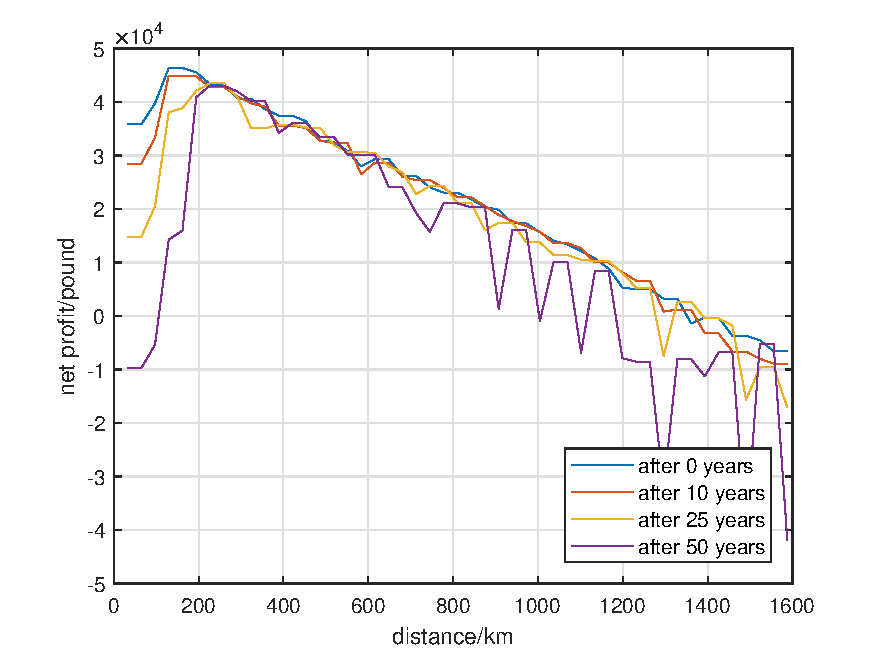
\includegraphics[width=3in]{image/distance_pro_qua.eps}
  %\caption{fig1}
  \end{minipage}%
  }%
  \subfigure[the elapsed time]{
  \begin{minipage}[t]{0.48\linewidth}
  \centering
  \includegraphics[width=3in]{image/ele_time_qua.eps}
  %\caption{fig2}
  \end{minipage}%
  }
  \centering
  \caption{profit graph}
\end{figure}

However, when the distance is more than 200 kilometers, due to the higher inherent cost of navigation, the fishing income will decline rapidly, showing a consistent downward trend among different years. At the same time, the 50-year net profit  curve fluctuated slightly compared to others due to the change in the position of fish density.

\section{Strategies we recommend}
\subsection{Using some proportion of small fishing vessels}

Assume that the fishing boat is a cuboid with a length of L, and its width and height are consistent with the previous assumptions.

Based on the data in Table 5, the power and mass corresponding to the different lengths of small fishing boats in Scotland are fitted to the relevant functional relations.The speed and flight time are calculated from the speed-related formula.
It is assumed that the operation of the refrigerant on the small fishing boat is supplied by the Scotland vessel, and that the refrigerator and engine at the same rated power consume the same amount of oil. Based on the density of the refrigerator, the price of diesel, and its comparison with the capacity of the vessel and its rated power, considering natural losses and energy conversion rates, it can be calculated that the operation of the refrigerant requires about 20\%  from the Scotland vessel the rated power

\begin{equation}\label{1}
v=1.84\times \ (\frac{P_0}{V}) ^{0.237} \times \sqrt{l}
\end{equation}

\begin{figure}[tbp]
  \centering{
  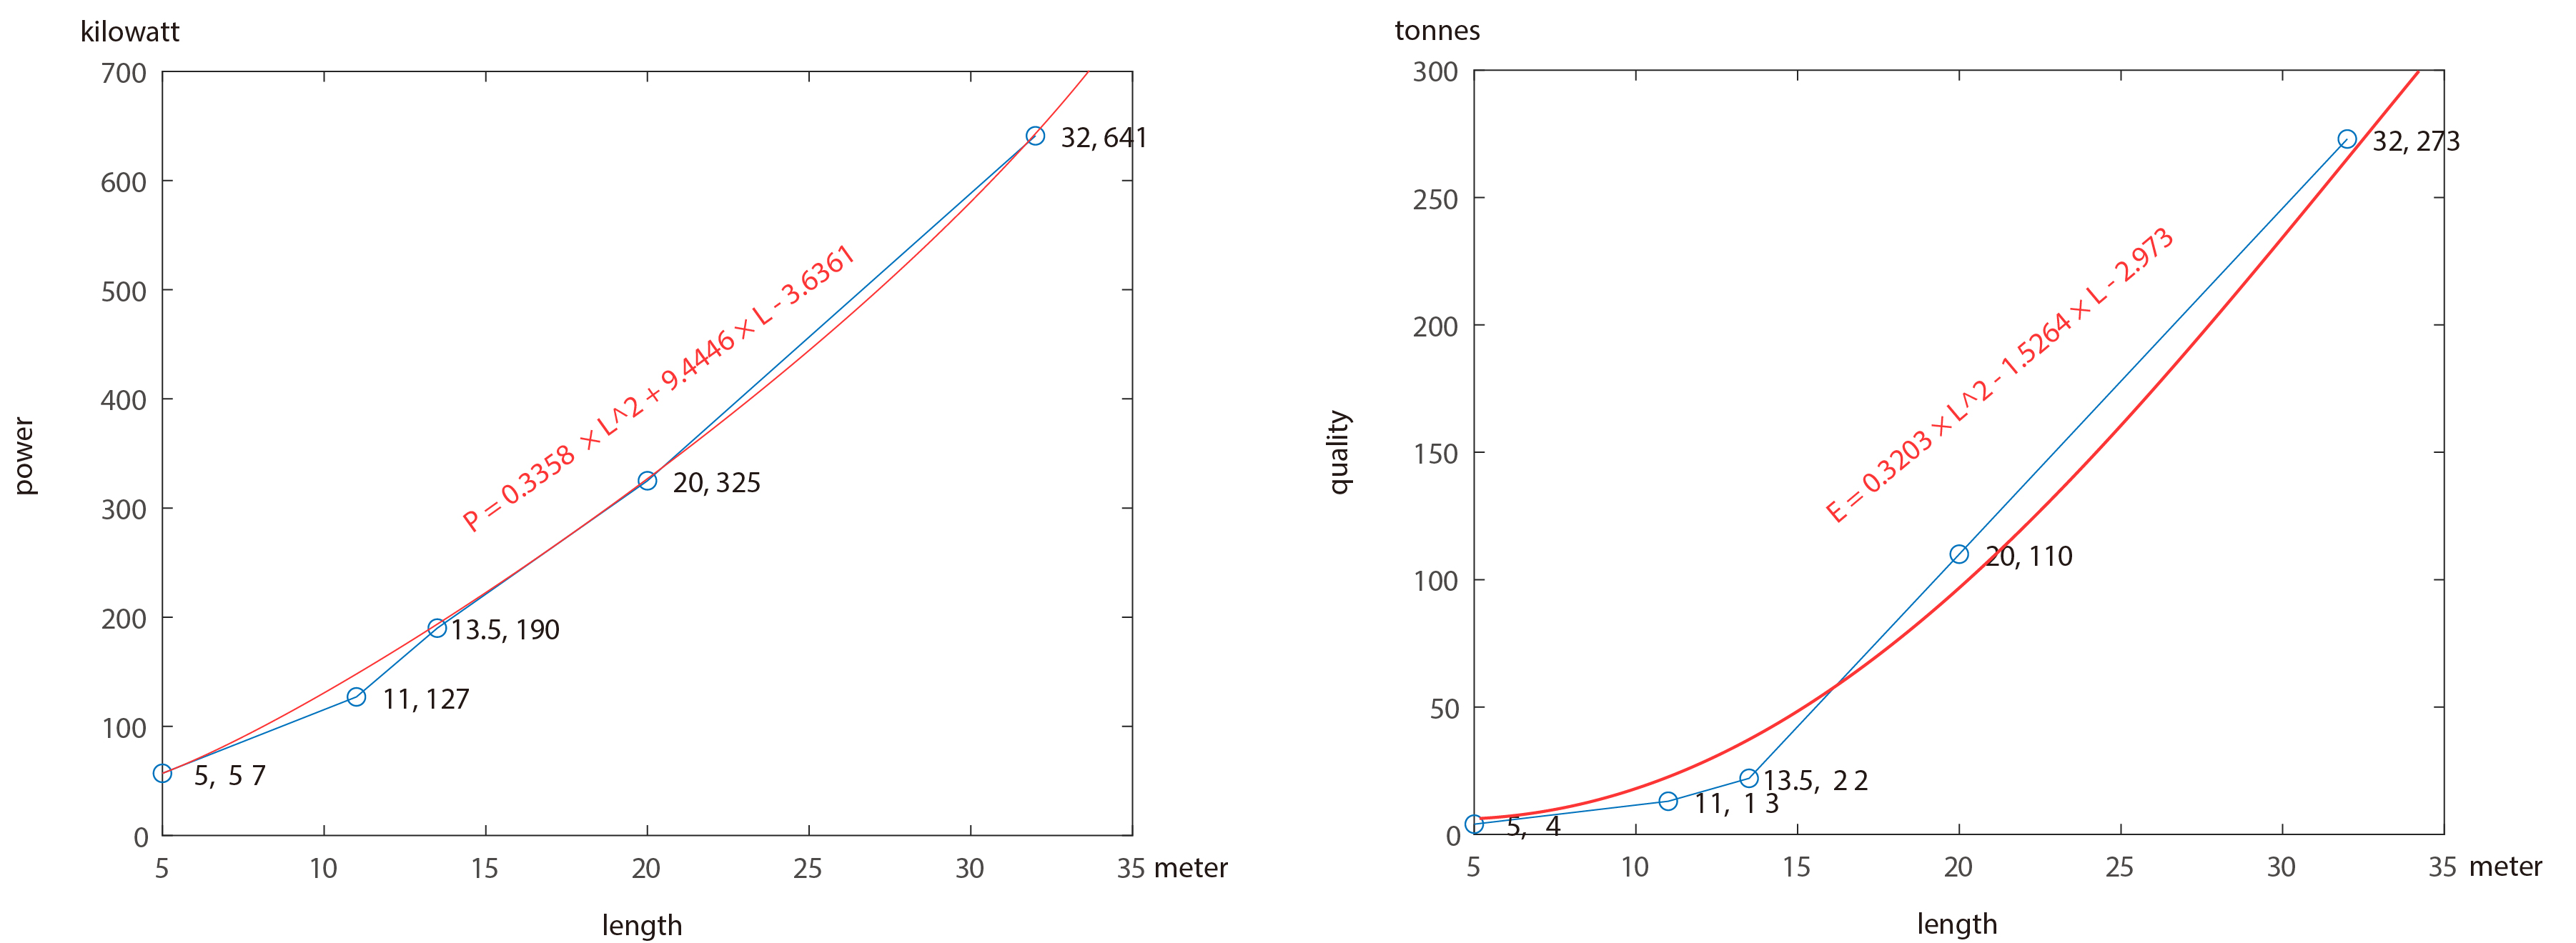
\includegraphics[width=1\textwidth]{./picture/figure4.jpeg}}
  \caption{The relationship between length and power and the relationship between length and quality }\label{figure1}
\end{figure}

\begin{equation}
\left\{
\begin{array}{lr}
P_0=P \times (1-20\%) &\\
P= 0.3358\times L^2 -9.4446\times L - 3.6361

\end{array}
\right.
\end{equation}



\begin{equation}\label{3}
V=L\times B\times\ d =\frac{1}{48\times L^3}
\end{equation}

\begin{equation}\label{4}
l=L\approx 40
\end{equation}

Due to the limitation of fuel storage space, fresh water, food and fishing supplies, it is assumed that the ship's navigation distance does not exceed fifth the original maximum navigation distance.

\begin{equation}\label{4}
T_1=\frac{S}{v}
\end{equation}

\begin{equation}\label{4}
S \leq 5\times S_m
\end{equation}

\begin{equation}
\left\{
\begin{array}{lr}
V_o=r_o \times P \times T_1 \times a_o &\\
a_o=0.8  & \\    p_o=0.5 \\
\end{array}
\right.
\end{equation}

By comparing the price of different sizes of refrigerants, it can be inferred that the cost of the refrigerant is about 10\% of the inherent cost of the ship. And both the labor cost and the inherent cost of the ship are positively related to the length of the vessel. Besides, due to the relocation of the port, the proportion of ships, the maintenance cost of the ship and the change in port charges $A_e$ in a single operation will decrease appropriately from 20,000 to 10,000 pounds. 

			\begin{equation}
			\left\{
			\begin{array}{lr}

A_1=c_3 \times T_1\times L \times (1+10\%) &\\
A_2=c_2  \times T_1 \times L \times  \frac{1}{2} &\\
A_3=V_o  \times P_o &\\
A=A_1+A_2+A_3+A_e \\		
			\end{array}
			\right.
			\end{equation}



\begin{equation}
\left\{
\begin{array}{lr}
E= -0.0175\times L^3 -1.2525\times L^2 - 15.197 \times L+ 51.952&\\
E_1=E \times 10\% \times a_1 \times p_1 &\\
E_2=E\times 10\% \times a_2 \times p_2 &\\
E= \frac{a_1 \times p_1}{a_1 \times p_1+ a_2 \times p_2} \times E_1 + \frac{a_2 \times p_2}{a_1 \times p_1+ a_2 \times p_2} \times E_2\\

\end{array}
\right.
\end{equation}

Then the profit graph change. In Figure 11 we can see small vessels Profit reduction rate reduce, but more importantly, small vessels (but not ) are capable of operating without land-based support, which mean they can go further to fish. In this way, they can reach the fish colony easily. 

\begin{figure}[htbp]
  \centering
  \subfigure[20m ship]{
  \begin{minipage}[t]{0.32\linewidth}
  \centering
  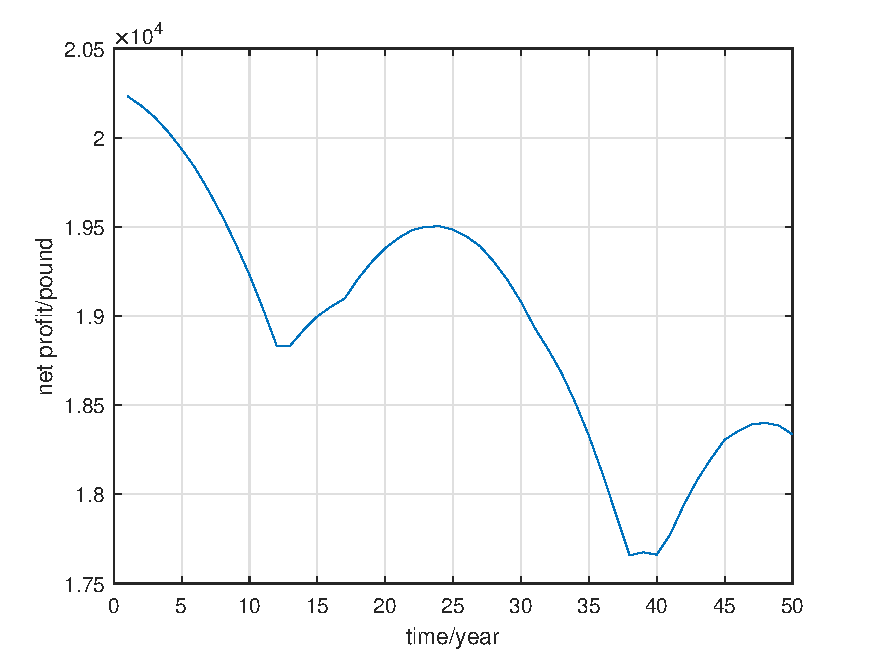
\includegraphics[width=2in]{picture/maxprofit_year_relation_ship20.eps}
  %\caption{fig1}
  \end{minipage}%
  }%
  \subfigure[15m ship]{
  \begin{minipage}[t]{0.32\linewidth}
  \centering
  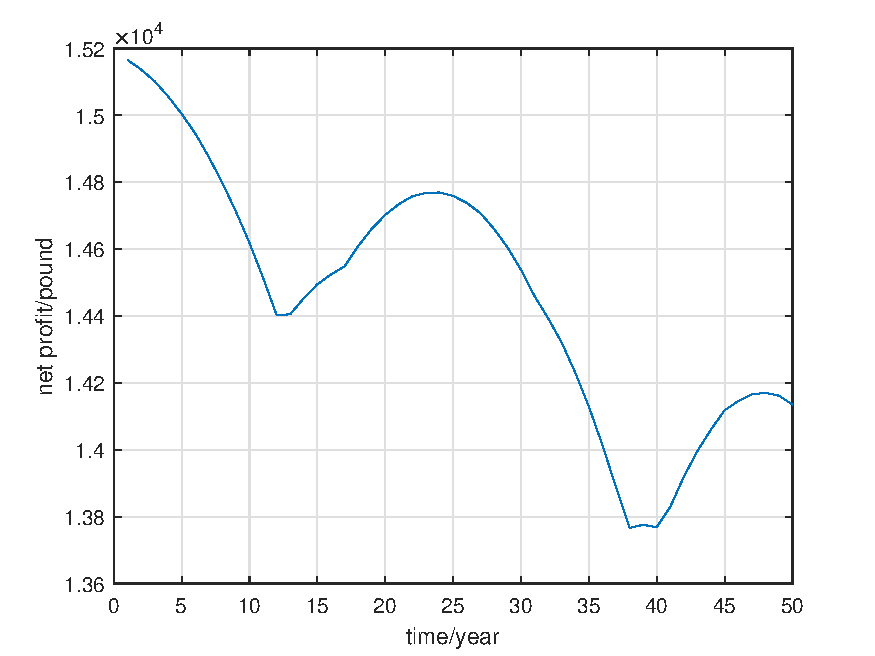
\includegraphics[width=2in]{picture/maxprofit_year_relation_ship15.eps}
  %\caption{fig2}
  \end{minipage}%
  }
  \subfigure[10m ship]{
  \begin{minipage}[t]{0.32\linewidth}
  \centering
  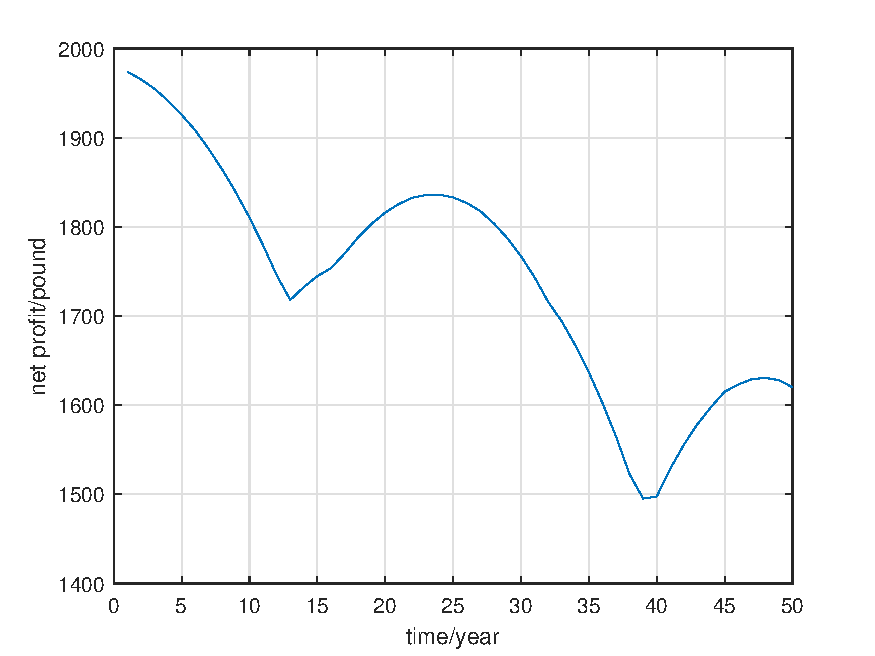
\includegraphics[width=2in]{picture/maxprofit_year_relation_ship10.eps}
  %\caption{fig2}
  \end{minipage}%
  }
  \centering
  \caption{Small vessels' profit graph}
\end{figure}


\subsection{Equip freezers for fishing vessels}
111

\begin{figure}[htbp]
  \centering
  \subfigure[the realationship between distance and net profit]{
  \begin{minipage}[t]{0.32\linewidth}
  \centering
  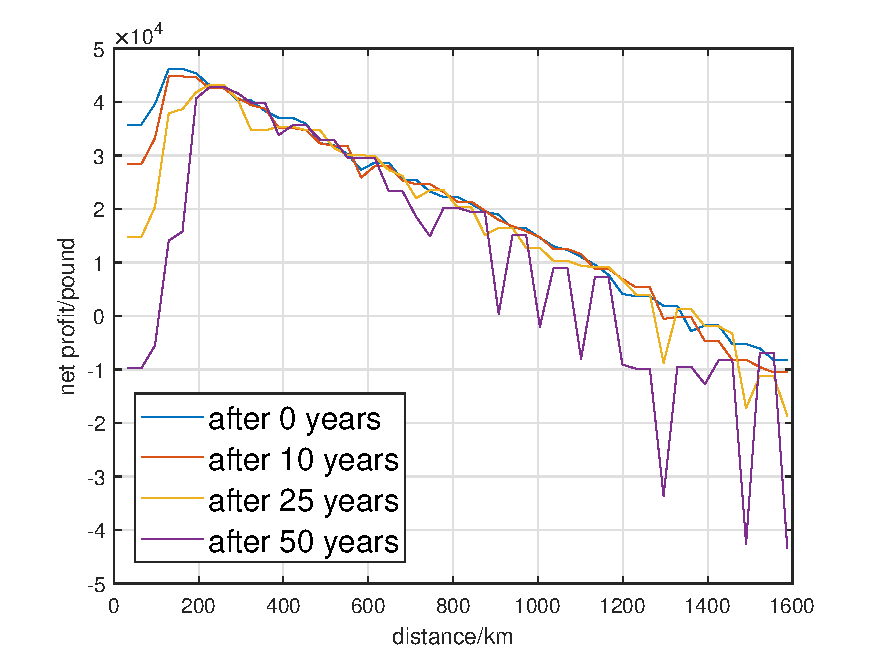
\includegraphics[width=2in]{picture/distance_pro__relation_ice.eps}
  %\caption{fig1}
  \end{minipage}%
  }%
  \subfigure[the elapsed time]{
  \begin{minipage}[t]{0.32\linewidth}
  \centering
  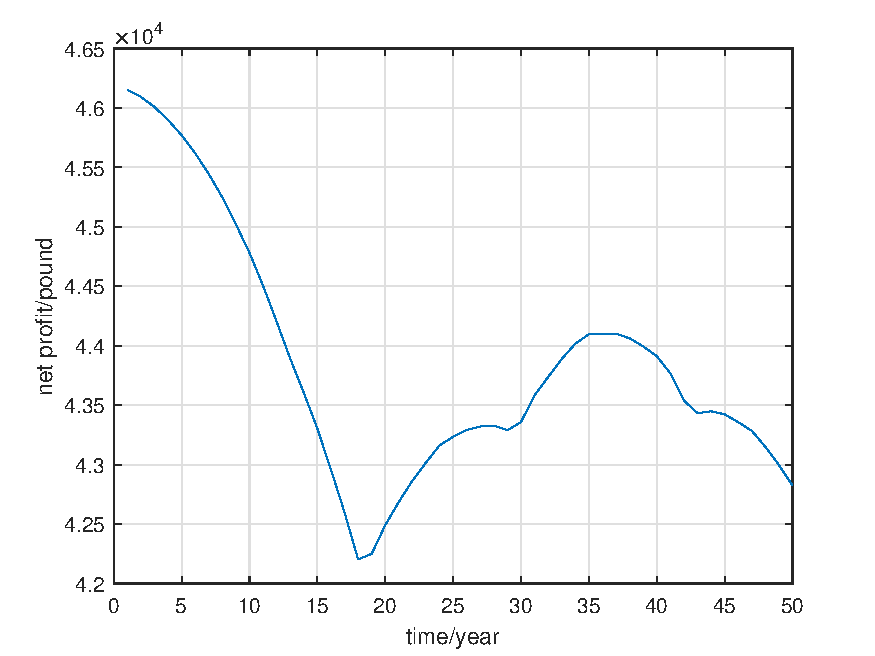
\includegraphics[width=2in]{picture/maxprofit_year_relation_ice.eps}
  %\caption{fig2}
  \end{minipage}%
  }
  \centering
  \caption{Vessels with freezers profit graph}
\end{figure}

\subsection{Relocate to other port}

222

\begin{figure}[htbp]
  \centering
  \subfigure[the realationship between distance and net profit]{
  \begin{minipage}[t]{0.32\linewidth}
  \centering
  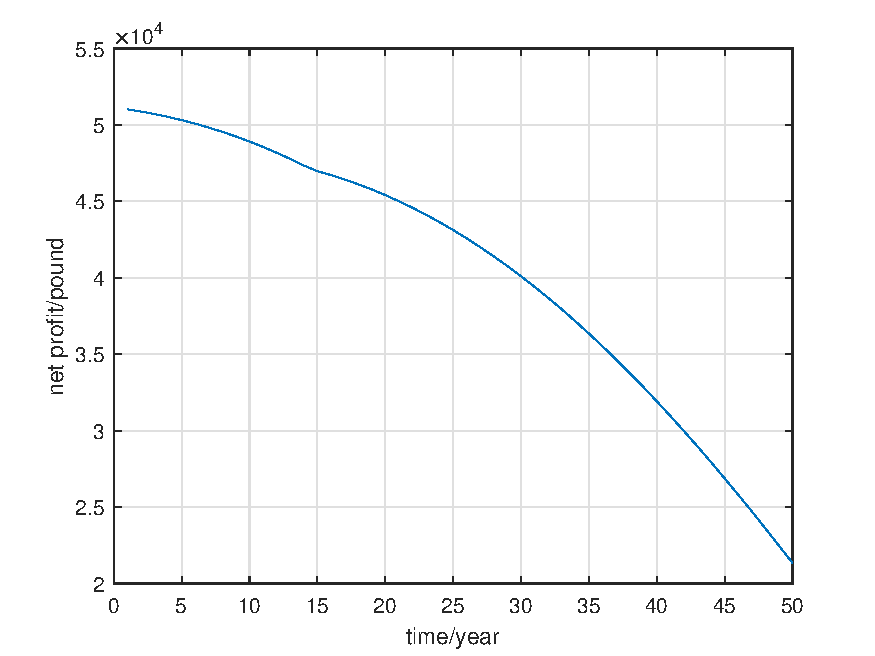
\includegraphics[width=2in]{picture/maxprofit_year_relation_change_port.eps}
  %\caption{fig1}
  \end{minipage}%
  }%
  \centering
  \caption{Vessels with freezers profit graph}
\end{figure}

\section{Model affected by territorial sea problem}
As can be known that territorial Waters is a belt of coastal waters extending at most 12 nautical miles (22.2 km) from the baseline (usually the mean low-water mark) of a coastal state, which are allowed innocent passage through it, or transit passage for straits.
It is assumed that the maritime division of the British Overseas Territories uses an equal distance method. As the waters of Scotland and Norway meet for 700 kilometers, it can be estimated that the range of Scottish fishing boats is within 350 kilometers.

\begin{equation}
\left\{
\begin{array}{lr}
A_i=A &\\
S_i \leq 350+22 =372 \\
\end{array}
\right.
\end{equation}



Assume that Norway ’s access fishing fee for foreign fishing vessels is the same as that of the member states of the Nauru agreement about 10,000 US dollars per day, which is 320 pounds per hour per boat. At the same time, due to Norwegian fishery restrictions, foreign fishing vessels can only sail in 12-200 nautical miles. Therefore, Scottish fishing boats have a range of 720 kilometers.

\begin{equation}
\left\{
\begin{array}{lr}
A_o=A+c_o \times T_3 &\\
T_3=\frac{S-S_i}{v} &\\
S_o \leq 350+370=720 \\
\end{array}
\right.
\end{equation}

For example, we use the vessels with freezers model and change the distance limitation to 372km (Figure 14 (a)), which means can't go into other territorial sea. Or we add the entry fee (Figure 14(b)), which means they go into other territorial sea. They both reduce profit.

\begin{figure}[htbp]
  \centering
  \subfigure[can't go into other territorial sea]{
  \begin{minipage}[t]{0.48\linewidth}
  \centering
  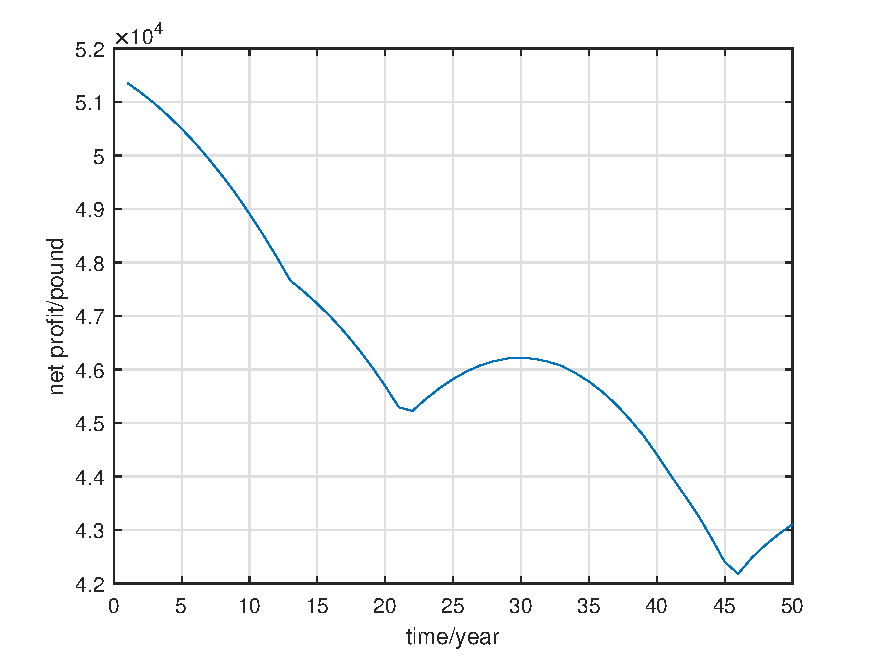
\includegraphics[width=3in]{picture/maxprofit_year_relation_ice_372.eps}
  %\caption{fig1}
  \end{minipage}%
  }%
  \subfigure[pay fee]{
  \begin{minipage}[t]{0.48\linewidth}
  \centering
  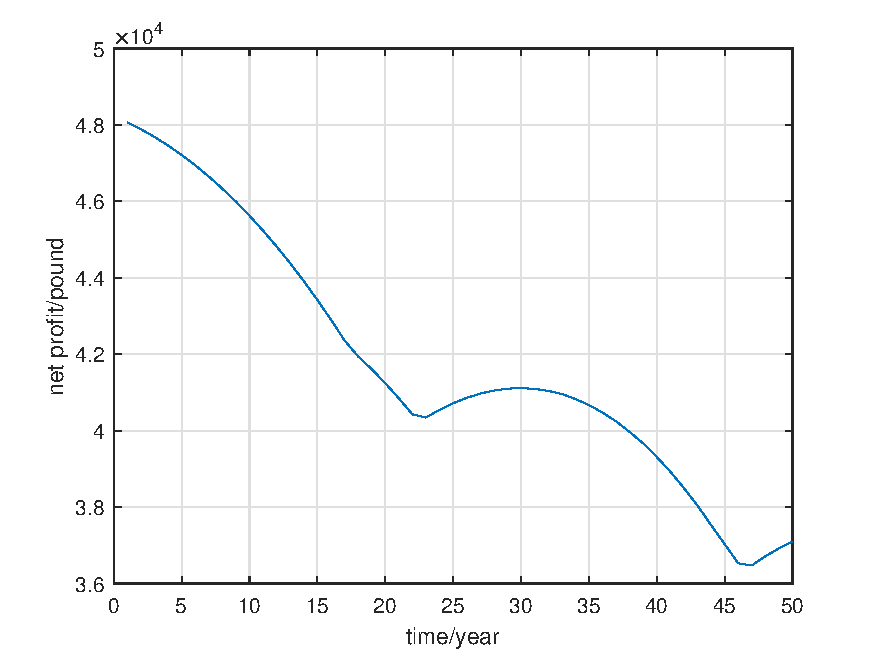
\includegraphics[width=3in]{picture/maxprofit_year_relation_change_port_2.eps}
  %\caption{fig2}
  \end{minipage}%
  }%
  \centering
  \caption{profit graph}
\end{figure}

\section{Sensitivity Analysis}
\subsection{}

figure~\ref{figure1}.

\section{Weaknesses and future improvements}

\begin{itemize}
  \item Most of the data we collected is average and may not be accurate.
   \item Without considering the interaction between the various coefficients, coefficient  are independent of each other
   \item To simplify the model, our assumptions ignore fishing time, speed change on return and the relationship between herring and mackerel.
     \item Without considering the detailed practical problems of the company location transfer.

\end{itemize}

Optimization method: When the forecast hat hurricane level is high, we can arrange inland evacuation ahead, in the case of ensure the overall time is enough for the coastal areas to evacuate to the site of the corresponding time calculation.

Advantage: Inland remove first can reduce the road pressure; Coastal remove later can increase the economic benefit. Compare the results again and get the final optimization plan.


\section{An article for Hook Line and Sinker magazine}
There are all kinds of interesting repertoires in the ocean at all times. We humans are not only spectators, but hunters. In the 21st century today, the ocean is our last hunting ground, and fishermen continue to bring food back to the whole society. According to statistics, 25\% of the proteins required by humans come directly from the ocean, and with the increase of the global population, this proportion will continue to rise, among which the most contributions are those rich fishing grounds.

For Scottish fishermen, herring and mackerel are gracious regulars in their lives. Mackerel is the most important pelagic species for the Scottish fishing industry. It is caught predominantly with pelagic trawl mainly in western waters and the North Sea.
At the same time , herring is the second most important species landed by the Scottish pelagic fleet. It has been one of the favorite fish in Europe for centuries, and there are many ways to eat outside of "street food ". For example, "Swedish herring can" has also become a Internet celebrity. herring is mainly caught for human consumption by vessels towing large pelagic mid-water trawls, with very little by-catch of other fish. 

Herring and mackerel are regulars on Scottish tables in that they are abundant, and the large number of herrings and mackerels also provide a good employment environment for Scotsman.

			\begin{figure}[htbp]
				\centering
				\begin{minipage}[c]{0.5\textwidth}
					\centering
					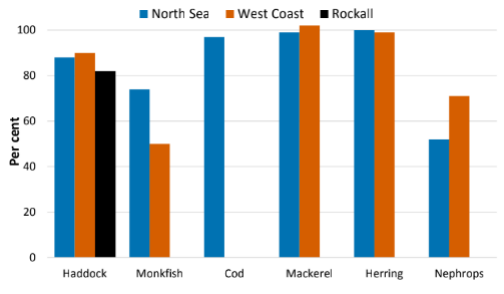
\includegraphics[width=9cm]{./picture/figure5.png}
				\end{minipage}%
				\begin{minipage}[c]{0.5\textwidth}
					\centering
					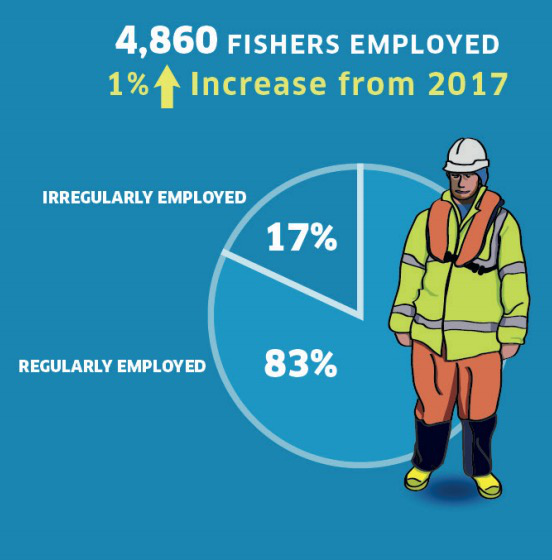
\includegraphics[width=4.5cm]{./picture/figure6.png}
				\end{minipage}
				\caption{Percentage quota uptakes of key commercial stocks by vessels in Scottish Producer Organizations in 2018}
			\end{figure}
			
The coat of fishing vessels are fixed expenditures. A fishing vessel costs hundreds of thousands of pounds. The maintenance of sailing is a relatively large expenditure. Compared with automobiles, the fuel consumption of boats is quite large. The rising oil prices have made shipowners miserable.
In addition to the basic equipment of fishing boats, port rents, access fishing fee, staff salaries, refrigerators are all huge expenses

Nowadays, due to over-fishing offshore and global warming, there are fewer and fewer fish  offshore, and fishermen have to go north to fish. The cost of equipment and labor has increased significantly. As the density of fish schools decreases, fishermen need to spend more time fishing. With the increase of time cost, fishing companies will use more professional and high-tech transport vessels, which is also a significant expense.


Therefore, we propose the following suggestions to ease or avoid the economic impact of fishing to global warming.

\begin{itemize}

\item 
Use the small size vessels
The small size vessels will reduce the cost of fishing and increase profits. For example, these short length vessels can get rid of restrictions from land-based support, such as refueling, unloading and so on. They can get those supplies from the large size vessels which might help fishermen to get the further areas to catch and net fishes.
\item
 Install the freezer
Freezers can extend the fish preservation time and greatly prolong the sailing time. Although the freezer also consumes the energy of the vessels, it can also allow fishermen to gain more profits.
\item 
Migration location
Relocating the fishing company to the location closer to the fish gathering point will  enable you to enjoy better fishing reduce economic losses(as can be seen in the figure ) 
\end{itemize}

Among the world's four major fisheries, Newfoundland fisheries have long lost their vitality due to overfishing. Peruvian fisheries focus on Peruvian catfish that have a poor taste and are mainly used as fodder. North Atlantic fishery nourished most of Europe, but in recent years the types of fishes in North Atlantic fishery have gradually decreased. 
The huge amount of carbon dioxide emitted by mankind contributes to global warming, and human greed puts marine life in a dangerous state. We should not only make corresponding economic policies for environmental changes, but also bear our responsibility for the current situation.

As you taste canned herring in Scotland, do not forget to thank these cute lives!







\addcontentsline{toc}{section}{Reference}
\bibliographystyle{plain}
\bibliography{myreference}

\begin{appendices}

\section{First appendix}

\lipsum[13]

Here are simulation programmes we used in our model as follow.\\

\textbf{\textcolor[rgb]{0.98,0.00,0.00}{Input matlab source:}}
% \lstinputlisting[language=Matlab]{./code/mcmthesis-matlab1.m}

\section{Second appendix}

some more text \textcolor[rgb]{0.98,0.00,0.00}{\textbf{Input C++ source:}}
% \lstinputlisting[language=C++]{./code/mcmthesis-sudoku.cpp}

\end{appendices}
\end{document}
